\documentclass[preprint,3p, 11pt,authoryear]{elsarticle}


\usepackage{graphicx}
\graphicspath{{./Graphic/}}
\usepackage{array}
\usepackage{amssymb} % various useful mathematical symbols
\usepackage{gensymb} % for `degree' sign
\usepackage{amsthm}  % extended theorem environments
\usepackage{lineno}   % for line numbers
\usepackage{tabularx} % for adjustable table width
\usepackage[hidelinks]{hyperref}  % for hyperlinks
\usepackage{amsmath}
\newtheorem{property}{Property}[section]
\usepackage{soul}
\usepackage{epsfig}
\usepackage{tabularx}
\usepackage{multirow} 
\usepackage{setspace}
\usepackage{adjustbox}
\usepackage{xcolor}
\usepackage[utf8]{inputenc}
\usepackage{mathrsfs}

\journal{Nondestructive Testing and Evaluation}

\begin{document}

\begin{frontmatter}



\title{A methodology for calculating active source-time functions from broadband piezoelectric sensors in the laboratory}

 \author[1]{Paul A. Selvadurai \corref{cor1}}
 \ead{paul.selvadurai@sed.ethz.ch}
\author[2]{Rui Wu}
\author[3]{Claudio Madonna}
\author[2]{Omid Moradian}




\cortext[cor1]{Corresponding author, Post-Doctoral fellow}
\address[1]{Swiss Seismological Service, ETH Zurich, Zurich, Switzerland}
\address[2]{Engineering Geology Group, ETH Zurich, Zurich, Switzerland}
\address[3]{Department of Earth Sciences, ETH Zurich, Zurich, Switzerland}



\begin{abstract}

\end{abstract}

\begin{keyword}
Acoustic emissions, physical acoustics, non-destructive testing, active source methods
\end{keyword}
\end{frontmatter}

\doublespacing
\linenumbers
\clearpage
%%%%%%%%%%%%%%%%%%%%%%%%%%%%%%%%%%%%%%%%%%%%%%%%%%%%%%%%%%%%%%%%%%%%%%%%%%%%%%%%%%%%%%%%%%%%%%%%%%%%%%%%%%%%%%%%%%%%%%%%%%%%%
\section{Introduction}
\label{int}

Understanding wave elastodynamic waves propagate through a medium has proven to have a multitude of applications in many fields of science and engineering.  
\\

Application in material science (crack detection), biomedics (ultrasonics), \textbf{more?} 
\\
The premise is to use well-understood physics associated with wave propagation, in fluids or solids media, to probe properties and assess its state in a non-destructive manner. 

\\\

The hope is to adopt techniques that have widely been used in the field of exploration geophysics in novel laboratories acoustic emission studies. To our knowledge, the benefits seen at scale from applications such as \textit{controlled-source interferometry} have not been fully explored in the laboratory with fully calibrated PZT actuator sources. We also see potential benefits when studying changes acoustic transmissivity \citep{PyrakNolte1980} with more accurate and coupled models that the simple linear slip model \citep[LSM,][]{Kendall1957}.  By understanding how various waves will be produced by our sensor (P and S waves) we can potentially understand the spatial variability in $V_{P}/V_{S}$ ratios to a higher degree of certainty. We foresee that an accurate transient force-time functions of our PZT actuators will help to frequently and non-invasively update time-dependent characteristics of the acoustic emission system component, such as: changes in passive transducer responses, in the transfer media or more accurate characteristics of similarly doublet events.  



\section{Experimental facilities}
\subsection{General}

We study elastodynamic waves propagating through an elastic isotropic, homogeneous steel plate. Using an electro-mechanical piezocomposite actuator, deliver impulsive sources on to the top surface of the steel specimen. On the bottom, an array of 13 piezoelectric (lead zirconate titanate, PZT) transducers are mounted in an aluminium array holder. The aim of this study is to better understand the force produced by the piezoelectric actuator by studying the waves produced at different locations on the bottom of the specimen.

Figure \ref{fig1}(a) shows a schematic representations of the steel platen (350 mm $\times$ 350 mm $\times$ 50 mm) in the extruded aluminium frame. Small rummer pads (10 mm $\times$ 10 mm $\times$ 1 mm) are used to base isolate the steel platen from the frame. Material properties of the steel plate required to model the wave propagation problem in the steel plate are given in Table \ref{table1}. Centrally located on the top surface is a piezoelectric actuator built in-house.  This sensor is connected to an high-voltage pulsing unit (HVP, Elsys Instruments AE-HV-MUX). This unit consist of a PiezosystemJena voltage amplifier for pulse generation (HVP 1000/200) that is fully integrated with the data acquisition (DAQ) software (Elsys Instruments TraNET). Figure \ref{fig1}(c) shows the circuit diagram of the HPV that is used to deliver an amplified voltage pulse to the piezoelectric actuator. The pulse and discharge of the system is depicted in the Figure \ref{fig1}(d). The time-dependent change in voltage when the switch position is in ``pulse'' (state 1) is given as:

\begin{equation}
\begin{array}{lcc}
  V(t) =  V_{0} \cdot \left[ 1 - exp\left(\frac{t}{R_{1}\cdot C_{PZT}} \right) \right], & \text{for} & 0 < t \leq t_{0}\\
\end{array}
\label{eq1}
\end{equation}

\noindent where $C_{PZT}$ = 300 pF, $R_{1}$ = 5 $\Omega$, $V_{0}$ = 200 V and the time of the pulse was set to $t_{0}$ = 1 $\mu$s. Discharging the systems required the switch to move to position 2 and we can solve for the theoretical discharge voltage:

\begin{equation}
\begin{array}{lclcc}
  V(t) =  V_{0} \cdot exp\left(-\frac{t - t_{0}}{R_{2}\cdot C_{eq}}\right), & \text{for} & t > t_{0}\\
\end{array}
\label{eq2}
\end{equation}

\noindent where $R_{2}$ = 1000 $\Omega$, $C_{eq}$ is the equivalent capacitance of $C_{PZT}$ and $C_{0}$ in series using electrostatic theory.  Figure \ref{fig1}(b) show the array holder for the passive sensor (KRNBB-PC) which are used to measure the stress waves produced by the active piezoelectric source. The aluminium array had a 7 $\time$ 7 locations with 23 mm spacing in both the $x$- and $y-$ directions.  In this study, we have assumed our source is symmetric about the $1-3$ and $2-3$ planes (i.e. aligned in the $3$-direction) and, therefore, have focused most of our sensors converge to one quadrant.  Similar colors of the sensors locations in Figure \ref{fig1}(b), represents similar epicentral locations.  We have redundant measurements at all epicentral locations expect $x$ = 0 mm, 33 mm and 96 mm and have shown that there appear to be little to no directivity in the active source.  

A total of 13 sensor are used and the spectral characteristics of these sensors have been well examined in the literature using the absolute calibration methods \citep{Glaser1998, McLaskey2010, McLaskey2012, Selvadurai2015, Selvadurai2019, Wu2020}. \citet{Glaser1998} provides a detailed account to sensor attributes used by KRN Services, including a the small field emission transistor (FET)-based Sanyo (2SK715W) preamplifier internal to the sensor casing to improve impedance matching.  These sensors have shown flat displacements-responses between 100 kHz to 1 MHz \citep{McLaskey2012, Selvadurai2019}.  At longer wavelengths between 1 kHz to 50 kHz these sensors have been found to behave more like accelerometer \citep{Wu2020}.

\begin{figure}[ht]
     	\centering
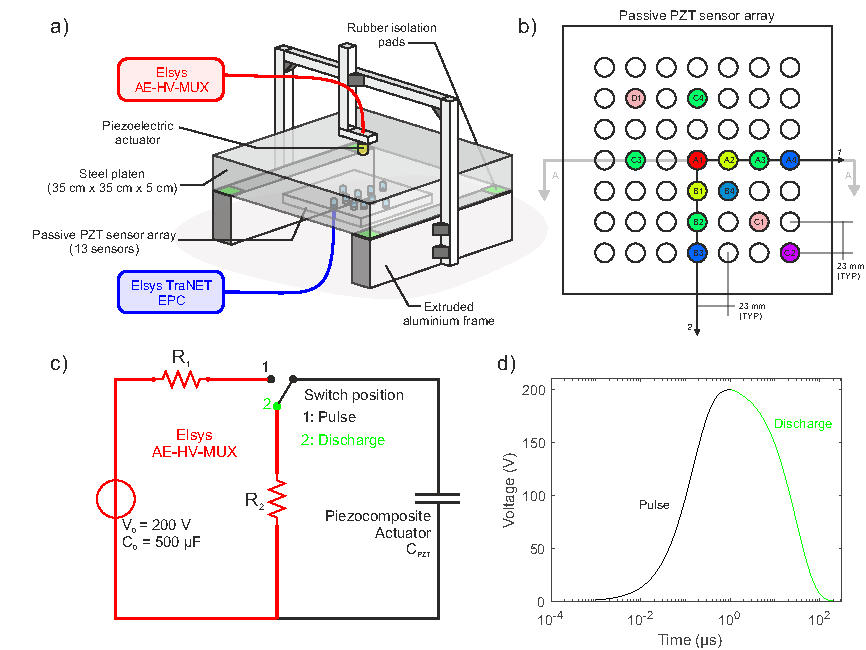
\includegraphics[scale= 1.0]{FIG1.pdf} 
\caption{\textbf{(a)} General schematic of the calibration station located in the Rock Physics and Mechanics Laboratory at ETH Zurich. We used apparatus to apply an active source downwards, which was centrally located on the top of a steel platen. This produced elastodynamic stress waves that are measured using an array of 13 broadband, passive PZT sensors. \textbf{(b)} The array of PZT sensors are shown where the colors indicate their epicentral location with respect to the source and is used throughout the study. \textbf{(c)} Driver circuit for pulse source diagram showing the elements associated with the Elsys high-voltage pulsing unit (AE-HV-MUX). \textbf{(d)} The solution for the time-dependent pulse and discharge of the voltage applied across the PZT element using circuit theory. }
	\label{fig1} 
\end{figure}

\begin{table}[ht]
	\centering
	\caption{Material properties of HABA CK45 steel test platen.}
	\begin{tabular}{ m{5cm} m{2cm} m{4cm}} 
		\hline  
		\bf{Parameter} 			& \bf{Symbol} 		& \bf{Value}	\\
	    Density                 & $\rho$            & 7850 kg/m$^{3}$\\
	    Shear modulus           & $\mu$             & 84 GPa \\
	    Poisson's ratio         & $\nu$             & 0.28\\
	    P wave velocity         & $V_{P}$           & 5890 m/s\\
	    S wave velocity         & $V_{S}$           & 3270 m/s\\	    
		\hline  	
	\end{tabular}
	\label{table1}
\end{table}

\subsection{Lamb's problem and PZT actuators}

The study of spherical waves in an elastic half-space was solved by \citet{Lamb1904} who was interested in the kinematic motions on a surface using the integral of plane waves solutions from \citet{Rayleigh1988}. More specifically, the Lamb's problem focuses on determining the elastic disturbance resulting from a point force in/on a half space. These early studies aimed at understanding phase arrivals and their relationship to earthquake sources in the field of seismology. These seminal investigations have been followed by many hundreds of studies that have use different mathematical approaches to solve the wave equation \citep[e.g. ch 6 in][]{Aki2002}.These studies vary in complexity in the media (in-homogeneous layered, or anisotropic, etc.), to complex source features (double couple, compensated-linear-vector-dipole, etc.) and use a range of different methods to solve (theoretical closed-form solutions, numerical methods, etc.). We adopt the approach presented by \citet{Johnson1974} that derived the complete solution to the three-dimensional Lamb’s problem derived using the Cagniard--de Hoop method. This solution is used to study the mechanical disturbances from sources in an elastic half-space and has been to a numerical generalized ray theory code by \citet{Hsu1985} \citep[see also][]{McLaskey2011, McLaskey2012, Selvadurai2019}.

While more complex sources have been considered to model earthquakes, such as the single and double couple source \citet{Sato1972}, we believe the original problem studied by \citet{Lamb1904} -- elastic displacements resulting from a point force in/on a half space -- is sufficiently complex for capturing the behavior of the piezoelectric actuator depicted in Figure \ref{fig2}(a). In Figure \ref{fig2}(a), we show the cross-section A-A from Figure \ref{fig1}(b). The source is produced by pulsing the piezoelectric actuator on the top surface using the experimental facilities described in Figure \ref{fig1}. The impulsive actuation of the PZT crystal on the steel plate produces a rapid transient source causing elastodynamic stress waves to propagate outwards. In Figure \ref{fig2}, the coloured region represents a synthetic representation of the velocity wave-field and is only provided as a reference and is not representative of the source produced from the PZT actuator (which is to be determined later). For this example, a snapshot of the velocity wave-field, produced from a capillary fracture is shown from numerical finite element simulations in ABAQUS \citep[adapted from fig. 2][]{Selvadurai2019}. 

Properties of the source creating the stress waves is important. \citet{Breckenridge1990} states that the ideal source is infinitesimal in size, has a force-time function of a step or delta function, and generates large amplitudes. He performed important study of a variety of sources including pencil lead fracture, capillary fracture, capacitive transducer, conical transducer, ball impact, spark, and high explosive, noting that each type is imperfect and has its trade offs. In this study, we look to aim to understand the PZT actuator (similar to conical transducer) which we can leverage to non-invasively study the \textit{in situ} absolute calibration conditions inside a less accessible experimental facility (e.g. trixaial pressure cell). To model the force-time function produced conical sensor, we first simplify the sequence of events and their components that link the source to the recorded signal.

In Figure \ref{fig2}(a), we show the five components of ``toolchain'' that is used to link the source to the measured signal. The PZT actuator is used to produce a (\textit{1}) \textbf{rapid transient force} $f_{j}$ on the top surface at a point $\mathbf{\xi}$ of the steel platen at a delayed time $\tau$. Elastic stress waves propagate through the plate and the theoretical elastic displacement field throughout the body can be computed using the (\textit{2}) \textbf{Green's function} $G_{kj}$. The Green's functions map the (\textit{3})\textbf{ elastic displacements} $u_{k}$ at $\mathbf{x}$ and time $t$ from the force at $\mathbf{\xi}$ and time $\tau$. A passive sensor, on the bottom surface at point $\mathbf{x}$ and attempts to measure the theoretical displacements $u_{k}$. Unfortunately, the passive sensors always will distort the (\textit{4}) \textbf{measured signal}  $s$ according to its (\textit{5}) \textbf{instrument response} $i_{k}$ at position $\mathbf{x}$ and time $t$.


developing more understanding of realistic force-time function produced by the PZT actuators has many potential benefits. Due to these properties we are able simply study and isolate individual components of the ``toolchain''. 

\begin{figure}[h]
     	\centering
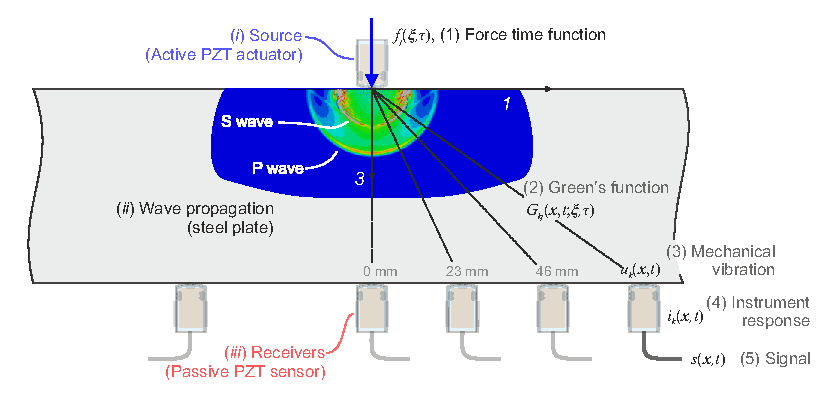
\includegraphics[scale= 1.0]{FIG2.pdf} 
\caption{Fundamental features related to the Lamb problem that relates elastodynamic displacements in an elastic half-space to a source (force-time) function. The velocity displacement field is shown for reference only and was adopted from \citet{Selvadurai2019}. P and S waves are highlighted for reference only. The PZT actuator is located centrally on the top of the steel plate and passive (recording) sensors are shown below for the Section A-A from Figure \ref{fig1}(b).}
	\label{fig2} 
\end{figure}


\section{Theoretical Framework}
\label{theo}

We build on the recent studies of signal analysis and instrument calibration by \citet{McLaksey2012} continuing this analysis using Green's function formalization \citep{Aki2002, Johnson1974}. Due to spatial reciprocity of the representation theorem \citep{Aki2002} and the invariant nature of the seismic wave equation to time-reversed solutions \citep{Fink1992}, we can use convolution of the components highlighted in Figure \ref{fig2} to analyze our system in a linear time-invariant (LTI) fashion. This assumes that changes in the sensor and source behavior and material properties are unaffected over time.  We assume point representations of both the sensor and source location, which might be influenced so-called ``aperture'' effect. However, this is minimized by using the point contact conical PZT crystal, which will be discussed later when we examine in more detail how the force systems of passive and active PZT sensors.

Using the classical theory describing dynamic elasticity \citep{Aki2002}, we can use Green's functions to relate the displacement $u$ at a known location $\mathbf{x}$ and time $t$ to a force $f$ at another point $\mathbf{\xi}$ and time $\tau$. This is given as the convolution of the force with the Green's function

\begin{equation}
\label{eq1}
           u_{k}\left( \mathbf{x}, t \right)  =  
            f_{j}\left( \mathbf{\xi}, \tau \right) \ast 
            g_{kj}\left( \mathbf{x}, t;\mathbf{\xi}, \tau \right).
\end{equation}
\noindent We note that $\ast$ represents convolution in the time domain, $f$ is the force acting in the $j$ direction at location $\mathbf{\xi}$ and $g_{kj}\left( \mathbf{x}, t;\mathbf{\xi}, \tau \right)$ is the elastodynamic Green's function describing the displacement $u$ in the direction $k$ at location $\mathbf{x}$. For the elastodynamic solutions studied here, we assume that convolution $\ast$ is applicable since the system in question are linear time-invariant (LTI) and that convolution has commutativity, associative and distributive properties. The true Green's function is the displacement field for the unit impulse force $\delta_{j}$ or the identity convolution. 

Piezoelectric transducers measure a voltage caused by the compression of the lead zirconate titanate (PZT) crystal in the surface normal direction $s\left( \mathbf{x}, t \right)$. We can relate the true surface displacement $u_{k}$ to voltage measurement $s$ using the instrument response, which is given as
   \begin{equation}
    \label{eq2}
        s\left( \mathbf{x}, t \right) =
            u_{k}\left( \mathbf{x}, t \right) \ast i_{k}\left(\mathbf{x},t \right).
    \end{equation}
    \noindent Combining \eqref{eq1} and \eqref{eq2}, we can represent the measured voltage to the forces which produced them:

    \begin{equation}
    \label{eq3}
        s\left( \mathbf{x}, t \right) =
            u_{k}\left( \mathbf{x}, t \right) \ast i_{k}\left(\mathbf{x}, t \right) =  
                f_{j}\left( \mathbf{\xi}, \tau \right) \ast 
                g_{kj}\left( \mathbf{x}, t;\mathbf{\xi}, \tau \right) \ast i_{k}\left(\mathbf{x},  t \right).
    \end{equation}

\noindent We can also use this formulation to relate the measured signals to a set of self-equilibrating forces or moments $m_{jp}$ \citep{Aki2002}. Displacements in the body are related to the spatial derivative of the elastodynamic Green's function $g_{kj,p}$.  While this is more similar to sources buried within a specimen and may be more representative of an earthquake source, this is not the focus of this study.  In this study, all sources are produced on the surface of the specimen, which justifies the use of only equation \eqref{eq2}.

\subsection{Time domain characteristics of the Force Function}
\label{force_time}

Our study aims at determining the nature of the dynamic transient source produced from the PZT actuator. We first decompose the source into two parts as shown here:

\begin{equation}
    \label{eq4}
    f_{j}\left( \mathbf{\xi}, \tau \right) =A_{0} \cdot f^{*}_{j}\left( \mathbf{\xi}, \tau \right) ,
\end{equation}

\noindent where $f^{*}_{j}$ is the normalized force-time function that has units (N) and a general shape to that follows the electro-mechanical behavior of the coupled high-voltage discharge and sensor systems.  A unitless scaling factor $\kappa(\tau)$ will be used to scale the normalized force time-function $f^{*}$ to the true force-time function $f$ and likely varies with the time as the electrical pulse is applied to the active source.

\begin{figure}[ht]
     	\centering
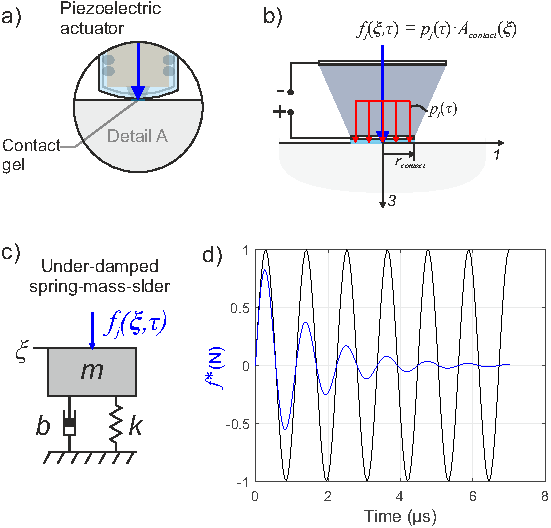
\includegraphics[scale= 0.9]{FIG2b.pdf} 
\caption{\textbf{(a)} Enhanced view of the contact region from the concial PZT actuator. \textbf{(b)} Simplified schematic showing the electro-mechanical systems and the estimate region where a pressure pulse $p_{j}$ (red) is generated when excited by the impulsive voltage. We assume that the force-time $f_{j}$ (blue arrow) is simply the integration of transient pressure over a constant circular contact area $A_{contact}$ and acting only in the 3-direction.  \textbf{(c)} Model summarizing the complex behavior of the PZT actuator (both internal and external) using an under-damped spring-mass damper systems whose behavior follow equation \eqref{eq4b}. \textbf{(d)} The normalized force-time function for: $A_{0}$ = 1 N, $\Gamma$ = 0 MHz and $\Lambda$ = 4.7 MHz (black line) and $A_{0}$ = 1 N, $\Gamma$ = 0.7 MHz and $\Lambda$ = 4.7 MHz (blue line).}
	\label{fig2b} 
\end{figure}

In Figure \ref{fig2b}(a) we look in detail at the position where the PZT actuator contacts steel plate. The actuator has threads on its body and is loaded on the plate by applying a small torque where the conical PZT tip is loaded through a thin layer of nickel (0.03 mm thick). This nickel foil is the cathode of the electro-mechanical circuit shown in Figure \ref{fig2b}(b), which represent a more detailed representation of the PZT actuator mentioned in the driver circuit (see Figure \ref{fig1}(c)). A small amount of contact gel is used to improve contact between the nickel cathode and steel plate but nickel was chosen due to is malleability and it formed a strong contact with the steel platen under minimal pressure \citep{Glaser1998}. To better understand the transient point force $f_{j}$ applied, we consulted literature in the biomedical industry that has studied piezomaterial, with similar pulsed excitation voltages, to perform ultrasonic reconstruction in acoustic media.  \citet{Christensen1988} looked at the pressure caused by a an electrical circuit that generated a sharp voltage pulse similar to that shown in Figure \ref{fig1}(d). Since the propagate waves through an acoustic medium they are interested in the time-dependent pressure boundary condition $p_{j}(\tau)$. To convert from pressure (over the tip area of the conical PZT) to an equivalent force $f_{j}$ we assume that the transient pressure field produced was uniform and therefore integrate over the contact tip area $A_{contact} = \pi r_{contact}^{2}$. For this PZT sensor the conical crystal has a contact radius of $r_{contact} = $ 0.75 mm. \cite{Christensen1988} found that the transient response of the pressure did not precisely duplicate the waveform of the voltage (see Figure \ref{fig1}(b)) due to the resonant properties of the crystal. When excited by a impulsive source, the crystal will resonate sinusoidal at its fundamental frequency and the wave will decay based in internal, external and transmitted losses.  The PZT actuator, when excited by the impulse, will produce a normalized pressure (or force-time function) described by the under-damped spring-mass damper system shown in Figure \ref{fig2b](c). \citet{Breckenridge1990} also showed evidence of under-damped behavior when exciting a conical PZT on an aluminium plate.

\citet{Christensen1988} notes that the damping of the pressure will be inversely proportional to the mechanical loss factor of the PZT crystal, but we argue that more variables might be contributing to this of the coupling of all the internal component such as the backing mass material and shape, they connections between the internal electrically conductive components, the shape of the crystal, the type of potting agent, the amount of coupling gel used, the type of material being pulsed (fluid or elastic), amongst other features \citep{Glaser1998}.  We argue that attempting to solve the full systems behavior with all these complexities is counter productive to the crux of this study. By the properties of convolution describing the wave propagation in equations \eqref{eq1}, we can assume that the measured signals will still have the general shape of the normalized force-time $f^{*}$ embedded in the measurements. We generalized the normalized force time function shown in Figure \ref{fig2b}(d) as follows

\begin{equation}
    \label{eq4b}
   f(t) = A_{0} \cdot exp[- \Gamma \cdot t]\cdot sin(\Lambda\cdot t) ,
\end{equation}

\noindent where $A_{0}$ = 1 N for the normalized case, $\Gamma$ and $\Lambda$ are the decay and vibration parameters of the normalized force-time function. We note that the subscript $_{j}$ has disappears since we are assuming that the normalized force is acting only in the $`3'$-direction. Later, we will describe how these two parameters are used in an inversion to minimize the errors between the theoretical displacements $u_{k}$ and measured signals $s$ over all the measured sensors. For the case in Figure \ref{fig2b}(d), $\Gamma$ = 0.7 MHz and $\Lambda$ = 4.7 MHz, which represented the best-fit solution for our analysis of the specific PZT used in this study following the excitation pulse in Figure \ref{fig1}(d).


\subsection{Calculating the Instrument Response}

We use properties of the Fourier transform \citep{Bracewell1986} to help deconvolve equations \eqref{eq3} and \eqref{eq4}.  In the frequency domain, convolution and deconvolution simply becomes multiplication and division. This allows us to isolate the components of interest we wish to quantify for our analysis. An example of the instrument response in the frequency domain $I_{w}$ simplifies to:

\begin{equation}
    \label{eq5}
        I_{k}\left(\omega \right) = 
        S\left( \mathbf{x}, \omega \right) \cdot \left[ F_{j}\left( \mathbf{\xi}, \hat{\omega} \right) \cdot G_{kj}\left( \mathbf{x}, \omega; \mathbf{\xi}, \hat{\omega} \right)\right]^{-1} .
\end{equation}

\noindent where $I_{k}$, $S$, $F_{j}$ and $G_{kj}$ are calculated from the temporal Fourier transforms of the $i_{k}$, $s$, $f_{j}$ and $g_{kj}$, respectively.  In a concerted study, we have predetermined the instrument responses for the exact same sensor configuration shown in Figure \ref{fig1}.  However, \citet{Wu2020} produced a known force-time function by dropping small steel balls of different diameters onto the surface from a known height at the identical location that will be used for the PZT actuator later. According to Hertzian contact theory, it is possible to assume a source time function that is a function of the material properties of the ball and steel platen ($E, \nu, \rho$), the radius of ball, and the drop height. This method has been popularized over the recent years due to a highly reliable and repeatable force-time function $f$ produced from ball impact and the ability to absolutely calibrate the acoustic emission sensors over a wide spectral range \citep{Breckenridge1990, McLaskey2010, McLaskey2012, McLaskey2015}. 

For the identical configuration of sensors shown in Figure \ref{fig1}(b), \citet{Wu2020} has dropped a range of small stainless steel (404) balls with diameters ranging from $d_{ball}$ = 0.3, 0.35, 0.4, 0.5, 0.6, 0.7, 0.8, 1.0, 1.5, 2.0 and 2.5 mm. The balls had elastic modulii of $E_{ball}$ = 210 GPa and Poisson ratio of $\nu_{ball}$ = 0.303, which allow them to calcaute the specific force-time function from Hertzian contact theory \citep[see also e.g.][]{McLaskey2010, McLaskey2012}. Once the force-time function is know, we use equation \eqref{eq5}, now with $F_{ball}\left( \mathbf{\xi}, \hat{\omega} \right)$, which represents the Fourier transform of the ball drop, to calculate the broadband instrument response $I_{k}(\omega)$ from 1 kHz to 1 MHz.  Calculating the lower frequency instrument response (i.e. 1 kHz to 50 kHz ) is not straightforward and the readers should also consult \citet{Wu2018} for a summary of methods. Figure \ref{fig6}(a) shows the full instrument response for all the passive sensors shown in Figure \ref{fig1}(b). The color coding related to the sensors epicentral distance from the ball drop source. In this study, we are only interested in the higher frequency (100 kHz to 1 MHz) sensor behavior for the reconstruction of the PZT actuator force time function. This range is shown in Figure \ref{fig6}(b). We see that the instrument response is insensitive to the take-off angle. This is important to the analysis and will be addressed in the more detail later. This insensitivity has also been acknowledged in the past for the same KRNPC-BB conical-style sensors used here \citep{Goodfellow2015, Selvadurai2019}.  Results from this calibration campaign are summarized and more details have been given in \citet{Wu2020}.


\begin{figure}[ht]
     	\centering
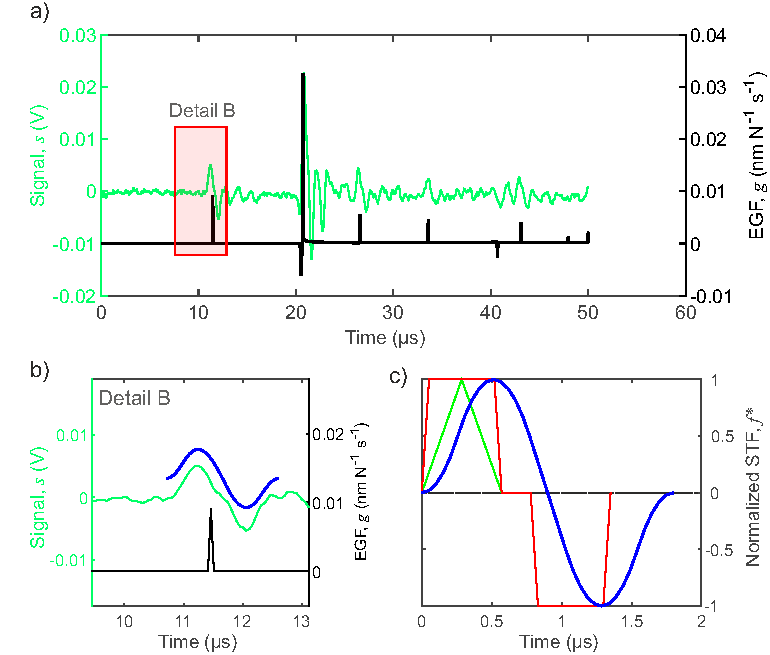
\includegraphics[scale= 1.0]{FIG6.pdf} 
\caption{Summary of the calibration experiments performed by \citet{Wu2020} to determine the instrument response for ball drops, performed \textit{a priori}, in the same location as where our PZT actuator was later placed. \textbf{(a)} The full range of calibrated frequencies (1 kHz to 1 MHz) is shown. \textbf{(b)} For our study, we only consider high-frequency aspect and therefore will only use the instrument responses between components 100 kHz to 1 MHz.  Colors are indicative of the sensors location as defined in Figure \ref{fig1}(b). For all the details please consult \citet{Wu2020}. }
	\label{fig6} 
\end{figure}

\subsection{Spectral Deconvolution of the Problem}

Having the specific broadband instrument response, solved using the well-understood ball drop source for our exact sensor-source layout, is paramount to accurately model the force-time function of the PZT actuator described by equation \eqref{eq4b}.   If we now consider the original problem in Figure \ref{fig2}, we can start with the recorded signal produced from the PZT actuator and use the instrument response to determined the mechanical vibration.  In the Fourier domain, we can rearrange the left hand side of equation \eqref{eq3} to estimate the spectral response of the theoretical vibration $U_{k}(\mathbf{x},t)$ caused by the transient PZT actuator:

\begin{equation}
    \label{eq6}
\begin{split}
U_{k}\left( \mathbf{x}, \omega \right) & = 
        \frac{S\left( \mathbf{x}, \omega \right) }{ I_{k}\left( \mathbf{x},\omega \right)}.
\end{split}
\end{equation}

Approaching the problem from the source side (right hand side of equation \eqref{eq3}), we can also estimate the mechanical vibration caused by the force of the PZT actuator convolved with the Green's function solution, which in the Fourier domain is shown as:

\begin{equation}
    \label{eq6a}
\begin{split}
U_{k}\left( \mathbf{x}, \omega \right) & = 
       F_{j}\left( \mathbf{\xi}, \hat{\omega} \right)  \cdot G_{kj}\left(  \mathbf{x}, \omega; \mathbf{\xi}, \hat{\omega}\right).
\end{split}
\end{equation}

\noindent Substituting the Fourier transform of the force-time function describe in equation \eqef{eq4}, we obtain

\begin{equation}
    \label{eq6b}
\begin{split}
U_{k}\left( \mathbf{x}, \omega \right) & = 
       A_{0}\cdot \delta (\omega)\cdot F^{*}_{j}\left( \mathbf{\xi}, \hat{\omega} \right)  \cdot G_{kj}\left(  \mathbf{x}, \omega; \mathbf{\xi}, \hat{\omega}\right),
\end{split}
\end{equation}

\noindent where the Fourier transform of the scaling parameter is $\mathcal{F}[A_{0}] = A_{0}\cdot\delta(\omega)$ and $\delta$ is the Dirac delta function.  Next we can combine equations \eqref{eq6} and \eqref{eq6b} to solve for the scaling factor for the force-time function $A_{0}$:


\begin{equation}
    \label{eq6b}
\begin{split}
A_{0} = \mathcal{F} ^{-1}[A_{0}\cdot \delta (\omega)] & = \frac{S\left( \mathbf{x}, \omega \right) } 
{ I_{k}\left( \mathbf{x},\omega \right)\cdot F^{*}_{j}\left( \mathbf{\xi}, \hat{\omega} \right)  \cdot G_{kj}\left(  \mathbf{x}, \omega; \mathbf{\xi}, \hat{\omega}\right)},
\end{split}
\end{equation}

\noindent where $\mathcal{F}^{-1}[\cdot]$  is the inverse Fourier transform. We see that all of the components on the right hand side can be measured ($S$) or calculated ($G_{kj}$) or have been determined \textit{a priori} ($I_{k}$) . We must assume that $A_{0}$ is constant over time and and the force-time function $f(\mathbf{\xi}, \tau)$, in equation \eqref{eq4b}, accurately captures the force released during the impulsive excitation of the PZT actuator. 

\section{Results}
\label{results}

In Figure \ref{fig3}(a) we show measurements on all passive sensors PZT sensors depicted in Figure \ref{fig1}(b).  Waveforms have been color coded following Figure \ref{fig1}(b) to show measurements taken at similar epicentral distances. These waveform we produced by actively exciting the source sensor located at the top central location of the steel platen. For our analysis, we only the first 50 $\mu$s of signal since we do not want to pollute the data with reflections from the boundary of the platen.  This allows us to analyze the wave using the approximation that the plate is in fact semi-infinite. Under this assumption we are able to solve for the Green's functions using the generalized ray theory code provided by \citet{Hsu1985} and modified for MATLAB by \citet{McLaskey2012}.  Figure \ref{fig3}(b) shows the Green's functions (EGF) at a give epicentral location from the source. We call this the empirical Green's function since it is a numerical approximation of the true Green's function that is the resulting ground displacements $u$ at point $\mathbf{x}$ from a unit impulse function $\delta_{j}(\mathbf{\xi}, \tau)$. In Figure \ref{fig3}(b) we also show the wave phase arrivals (P, S, PPP, PPPPP) for the numerical models.

\begin{figure}[ht]
     	\centering
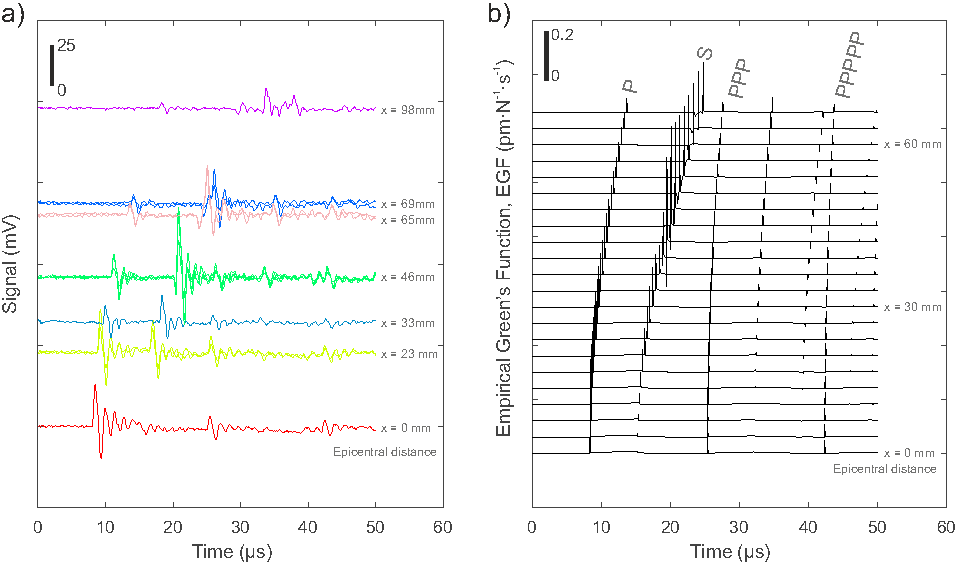
\includegraphics[scale= 1.0]{FIG3.pdf} 
\caption{\textbf{(a)} Measurements the array of passive PZT transducers from a PZT actuator source described in Figure \ref{fig1}(d). The color scheme represents the different epicentral locations of each sensor in Figure \ref{fig1}(b).  \textbf{(b)} Green's function solutions using generalized ray theory for a semi-infinite elastic, homogeneous steel plate at different epicentral locations.  The empirical Green's function (EGF) is the numerical estimate of the true Green's function, which is displacements produced from the unit impulse force $\delta_{j}(\mathbf{\xi}, \tau)$. We see the various phase arrival predicted from the model.}
	\label{fig3} 
\end{figure}

Figure \ref{fig4} compares the theoretical Green's function $g_{kj}$ to the measured signals $s$.  For clarity, we only show the sensors A1 (red), A2 (yellow), A3 (green) and A4 (blue) from the epicentral distances of 0 mm, 23 mm, 46 mm and 69 mm, respectively. We see that the sensors appear to capture the multiple phase arrivals and this is believed to be due to the conical nature of the PZT crystal and its ability to capture wave arrivals at high azimuthal incident angles \citep{Selvadurai2019}. Results in Figure \ref{fig4} are representative of the measurements across all 13 passive sensors.

\begin{figure}[ht]
     	\centering
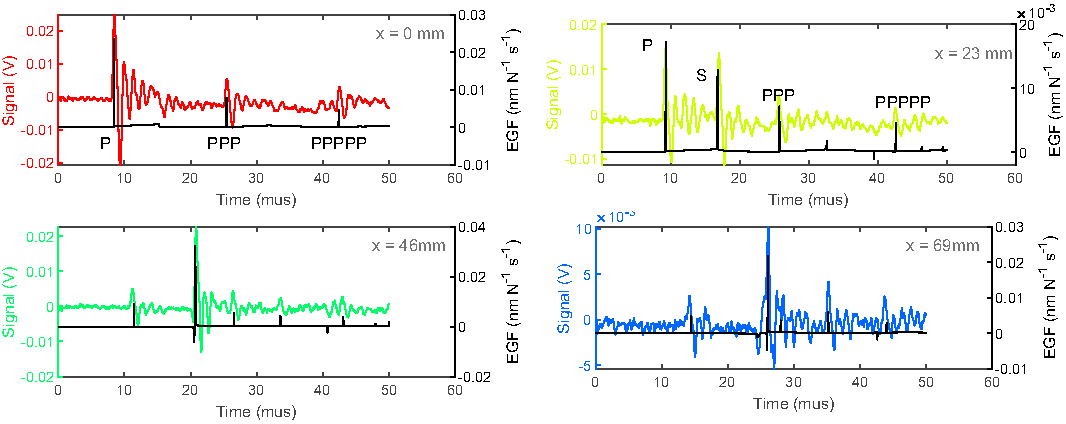
\includegraphics[scale= 0.90]{FIG4.pdf} 
\caption{Comparison of measurements on sensors A1, A2, A3 and A4 to the emipircal Green's functions calculated using generalized ray theory. The KRNBB sensor perform well and capture the wide range of wave phase arrivals.}
	\label{fig4} 
\end{figure}

To best show the approach we take to solve for the force time function produced by the active source, we focus on the measurements taken from sensors A3 at epicentral distance $x$ = 46 mm. Figure \ref{fig5}(a) shows the measurements and EGFs.  We focus on detail B, which looks at the first arrival P wave.  In Figure \ref{fig5}(b) this is shown in more detail with the sensors (green trace) and EGF (black trace) clearly visible.  Since we know that, in the time domain, the signal produced on the sensors the force-time function are convolved with the associated Green's function, the shape of the specific wave with be representative of the source. The blue curve in Figure \ref{fig5}(b) is a best-guess approximation of the source and will be use to estimate the general normalized force-time function $f^{*}_{j}$ from equation \eqref{eq4}.

\begin{figure}[ht]
     	\centering
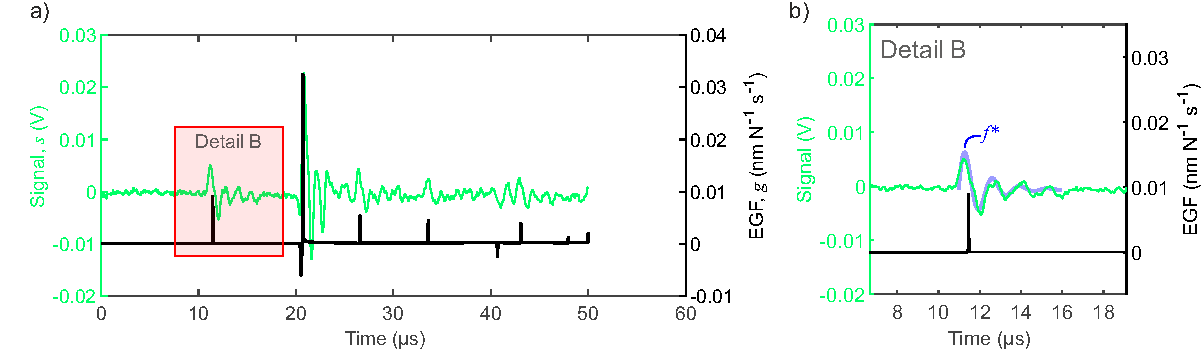
\includegraphics[scale= 0.85]{FIG5.pdf} 
\caption{\textbf{(a)} Measurements from sensor A3 (green line) from the active source compared to the EGFs at the same place from the model.  Detail B looks more closely at the first-arrival P wave. \textbf{(b)} Shows the general shape of the P wave (green line) versus the location of the expected P wave arrival (black line) form the Green's function solution.  From the convolutional nature of the wave propagation problem (equation \eqref{eq1}) we can estimate the general shape of the normalized force-time function $f^{*}_{j}$ shown as the blue line.}
	\label{fig5} 
\end{figure}

 We created the normalized force-time function based on characteristic of the first arrival P wave.  In Figure \ref{fig5}(c) we show the methodology for generating $f^{*}_{j}$.  We based this on the technical specifications of the high-voltage pulsing unit described in Section \ref{XXX}. In this experiment we applied a 100V pulse, which translates into a positive pulse, followed by a delay, then a negative pulse.  We approximated this behavior using piecewise discontinuous step functions (red curve) that was convolved with a 0.6 $\mu$s triangle function to smoothen the step function. This produced the blue curve which matched the general shape of the P wave arrival in Figure \ref{fig5}(c).  We will use this as a forward model to approximate the source-time from the active PZT source. We clearly see that the normalized force-time function varies from [-1,1], which is appropriate for our definition of $f^{*}$ in Section \ref{XXX}.



To solve for the scaling function $K(\hat{\omega})$ we need to know the instrument response function $i(t)$. For this study, we use the results from \citet{Wu2020}. They performed multiple ball drops to create known force-time functions at the same location as the active sensors. The same sensors were used in their study and a series of different ball sizes where used (diameters = 0.3 mm, .....to 1.5 mm).  \citet{Wu2020} modeled long times to also capture how the sensors responded to frequencies as low as $f$ =1 kHz, following the methodology by \citet{Wu2018}.  Figure \ref{fig6}(a) shows the full instrument response function for each sensor in the Fourier domain (see equation \ref{eq5}).  Figure \ref{fig6}(b) focuses only on the results for frequencies between $f$ = 100 kHz to 1000 kHz, which is more important to our understanding of the true force-time function in our case.  



\begin{figure}[ht]
     	\centering
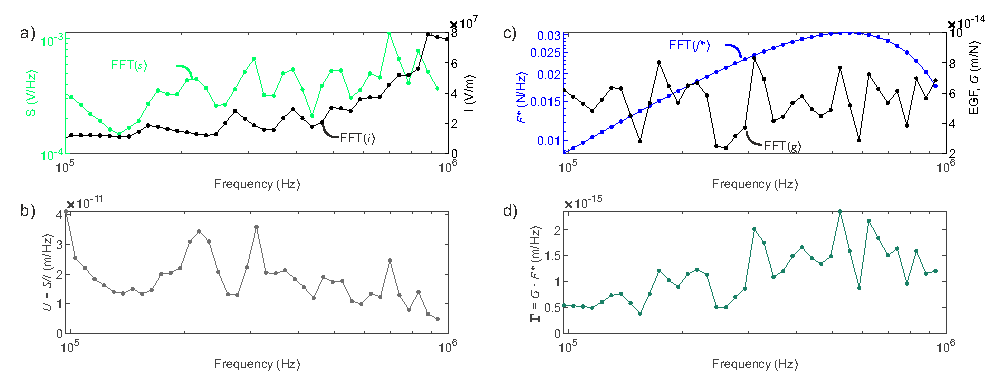
\includegraphics[scale= 1]{FIG7.pdf} 
\caption{\textbf{(a)}  }
	\label{fig7} 
\end{figure}


\begin{figure}[ht]
     	\centering
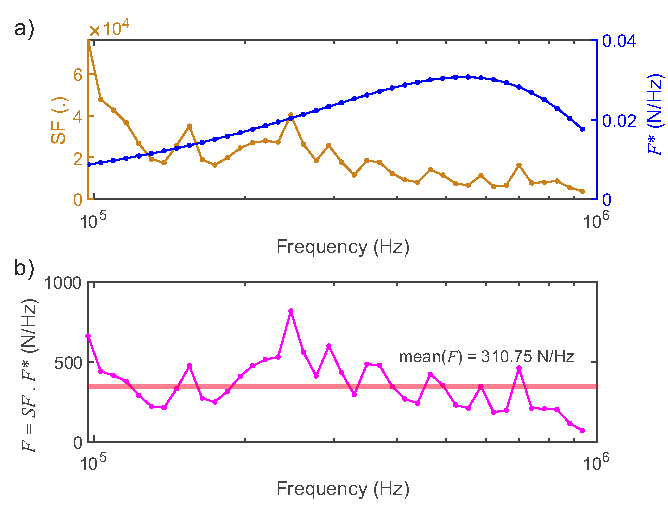
\includegraphics[scale= 1]{FIG8.pdf} 
\caption{\textbf{(a)}  }
	\label{fig8} 
\end{figure}


\begin{figure}[ht]
     	\centering
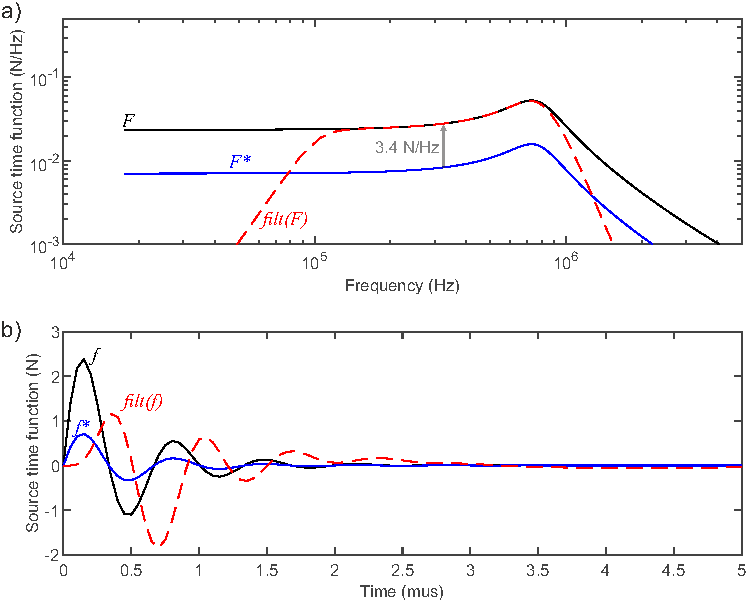
\includegraphics[scale= 1]{FIG9.pdf} 
\caption{\textbf{(a)}  }
	\label{fig9} 
\end{figure}

\begin{figure}[ht]
     	\centering
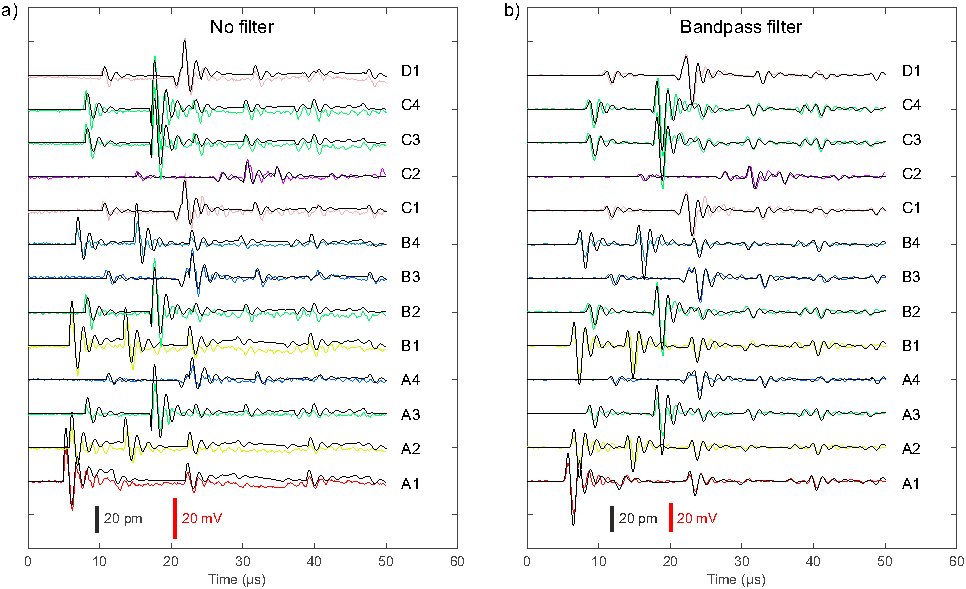
\includegraphics[scale= 1]{FIG10.pdf} 
\caption{\textbf{(a)}  }
	\label{fig10} 
\end{figure}




\clearpage

\section*{Acknowledgement}
T. M\"orgeli
 

\bibliographystyle{elsarticle-harv} 
\bibliography{Source_reconstruction}


\section*{Supplemental information}


\begin{table}[ht]
	\centering
	\caption{Material properties of Piezoelectric active source (PZT-5A).}
	\begin{tabular}{ m{5cm} m{2cm} m{4cm}} 
		\hline  
		\bf{Parameter} 		      & \bf{Symbol} 	  & \bf{Value}	\\
	   & \textit{Mechanical properties} & \\
	    Density                   & $\rho$            & 7500 kg/m$^{3}$\\
	    Poisson's ratio           & $\nu$             & 0.31\\
	    Young's modulus           & $E$               & 66 GPa\\
        Curie Point               & $T_{c}$           & 350 $^{o}$C\\  
        Mechanical quality factor &   $Q_{m}$         & 100\\
	  & \textit{Piezoelectric constants} & \\
 	  & d_{33}                   & 3.74 $\times$ 10$^{-10}$ m/V\\
 	  & d_{31}                   & -1.71 $\times$ 10$^{-10}$ m/V\\
	  & \textit{Dielectric constants} & \\
 	  & d_{33}                   & 3.74 $\times$ 10$^{-10}$ m/V\\
 	  & d_{31}                   & -1.71 $\times$ 10$^{-10}$ m/V\\

	       
		\hline  	
	\end{tabular}
	\label{table1}
\end{table}



\end{document}
\endinput
